\documentclass[onecolumn,aps, pre,amsmath,amssymb,longbibliography,11pt]{revtex4-2}
\usepackage{graphicx}
% \usepackage{dcolumn}
\usepackage{bm}
\usepackage{amsfonts}
\usepackage{xcolor,tabu}
\usepackage{multirow}
\usepackage{amsthm}
\usepackage{textcomp}
\usepackage{tikz}
\usepackage[colorlinks=true,
            linkcolor=blue,
            urlcolor=blue,
            citecolor=blue]{hyperref}
\hypersetup{bookmarksopen=true}
\usepackage{xr}
\usepackage{float}



\begin{document}
\title{Numerical Solution of Poisson Equation}

\author{Zhengyang Liu}
\date{\today}
\maketitle

This note documents the numerical solution of Poisson Equation. Consider the following PDE
\begin{equation}\label{eq:poisson}
\nabla^2\psi(x, y) = -\omega
\end{equation}
in domain $x, y \in [0, 1]$.

We start by discretizing the Laplacian $\nabla^2\psi$ in Eq.~\ref{eq:poisson} using the centered difference approximation, into an $N\times N$ grid. The distance between adjacent grid nodes is $h=1/N$. \textcolor{red}{Other higher order discretization schemes will be discussed later.}
%
$$
\left(\frac{\partial\psi}{\partial x}\right)_{i, j} \approx (\psi_{i+1, j} - \psi_{i, j}) / h
$$
$$
\left(\frac{\partial\psi}{\partial x}\right)_{i-1, j} \approx (\psi_{i, j} - \psi_{i-1, j}) / h
$$
\begin{equation}\label{eq:x-approx}
\begin{split}
\left(\frac{\partial^2\psi}{\partial x^2}\right)_{i, j} & \approx \left(\left(\frac{\partial\psi}{\partial x}\right)_{i, j} - \left(\frac{\partial\psi}{\partial x}\right)_{i-1, j}\right)/ h \\
 & = \frac{(\psi_{i+1, j} - \psi_{i, j}) / h - (\psi_{i, j} - \psi_{i-1, j}) / h}{h} \\
 & = \frac{\psi_{i+1, j} - 2\psi_{i, j} + \psi_{i-1, j}}{h^2}
\end{split}
\end{equation}
%
similarly,
\begin{equation}\label{eq:y-approx}
\left(\frac{\partial^2\psi}{\partial y^2}\right)_{i, j} \approx \frac{\psi_{i, j+1} - 2\psi_{i, j} + \psi_{i, j-1}}{h^2}
\end{equation}
combine Eqs.~\ref{eq:x-approx} and \ref{eq:y-approx}, we get
\begin{equation}\label{eq:discrete-laplacian-approx}
(\nabla^2\psi)_{i, j} = \frac{\psi_{i+1, j} + \psi_{i, j+1} - 4\psi_{i, j} + \psi_{i-1, j} + \psi_{i, j-1}}{h^2} = -\omega_{i, j}
\end{equation}
%
For each node $(i, j)$, there is a linear equation of $\bm{\Psi}=(\psi_{0, 0}, ..., \psi_{N-1, N-1})$. These equations form a linear system with $N\times N$ equations, where $\bm{\Psi}$ can be solved for.
%
\begin{figure}[h]
\begin{center}
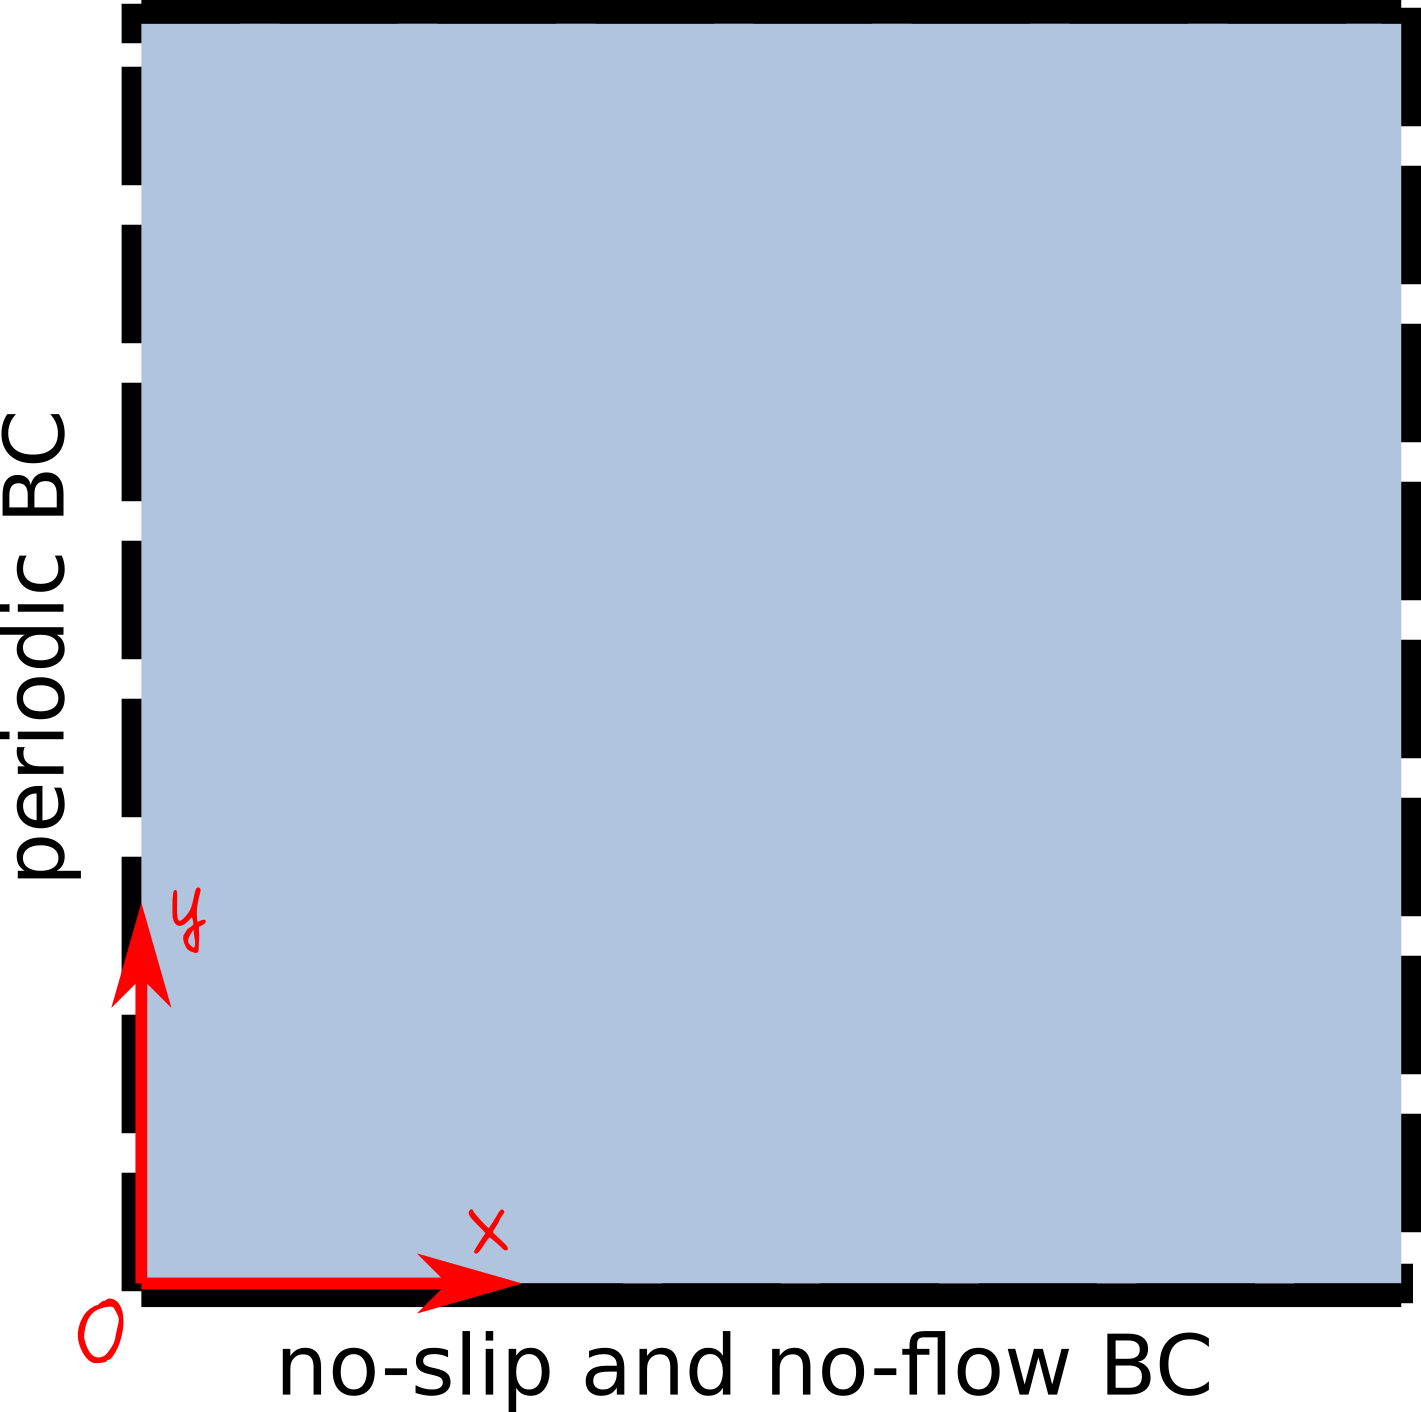
\includegraphics[width=3in]{Figures/schematic.svg.png}
\caption[Schematic]
{
Schematic of the system.
}
\label{fig:schematic}
\end{center}
\end{figure}
%
The linear system can be expressed in the form of $\bm{Ax}=\bm{b}$, where
\begin{equation}\label{eq:linear-system}
\bm{A} = \begin{bmatrix}solution
    \ddots & & & & & & & &  \\
           & \ddots & & & & & & &  \\
           & & \ddots & & & & & &  \\
           & & & \ddots & & & & &  \\
    \dots & 1 & \dots & 1 & -4 & 1 & \dots & 1 & \dots \\ % 5
    & & & & & \ddots & & &  \\
    & & & & & & \ddots & &  \\
    & & & & & & & \ddots &  \\
    & & & & & & & & \ddots \\
  \end{bmatrix}_{N^2\times N^2}
    , \
\bm{x} = \begin{bmatrix}
    \vdots \\
    \psi_{i-1, j} \\
    \vdots \\
    \psi_{i, j-1} \\
    \psi_{i, j} \\
    \psi_{i, j+1} \\
    \vdots \\
    \psi_{i+1, j} \\
    \vdots
  \end{bmatrix}_{N^2}
\end{equation}
%
The row shown in $\bm{A}$ is the $(iN+j)$ th row, corresponding to the $(i, j)$ element in the discretized streamfunction $\psi$ and vorticity $\omega$. Multiplying this row to $\bm{x}$, we backup the general form of Eq.~\ref{eq:discrete-laplacian-approx}. Note that near the boundaries, this general form needs to be modified to satisfy the boundary conditions. This is what we are going to do next.

\textbf{Boundary conditions} \\ [1em]

As in Fig.~\ref{fig:schematic}, we impose periodic boundary condition in $x$ direction and no-slip-no-flow boundary condition in $y$ direction. The no-slip-no-flow boundary condition is formally stated as
% %%%%%%%%%%% This is not the right way to impose periodic BC
% $$%%%%%%%%%%%%%%%%%%%%%%%%%%%%%%%%%%%%%%%%%%%%%%%%%%%%%%%%%
% \psi\Big|_{x=0} = \psi\Big|_{x=1}%%%%%%%%%%%%%%%%%%%%%%%%%%
% $$%%%%%%%%%%%%%%%%%%%%%%%%%%%%%%%%%%%%%%%%%%%%%%%%%%%%%%%%%
% %%%%%%%%%%%%%%%%%%%%%%%%%%%%%%%%%%%%%%%%%%%%%%%%%%%%%%%%%%%
$$
\frac{\partial\psi}{\partial y}\Big|_{y=0}=\frac{\partial\psi}{\partial y}\Big|_{y=1}=\frac{\partial\psi}{\partial x}\Big|_{y=0}=\frac{\partial\psi}{\partial x}\Big|_{y=1}=0
$$
%
The periodic boundary condition, to my knowledge, can only be expressed in a discretized expression.

Now let's discretize the boundary conditions. Here, we consider the conditions at $y=0$ a backward discretization and the conditions at $y=1$ a forward discretization. The idea is to use the BC's to generate extra ``imaginary grids'' so that the Laplacian at the boundaries can be evaluated more accurately. Fig.~\ref{fig:im-grid} shows how an imaginary node $(-1, j)$ helps evaluating the Laplacian at $(0, j)$.
%
\begin{figure}[h]
\begin{center}
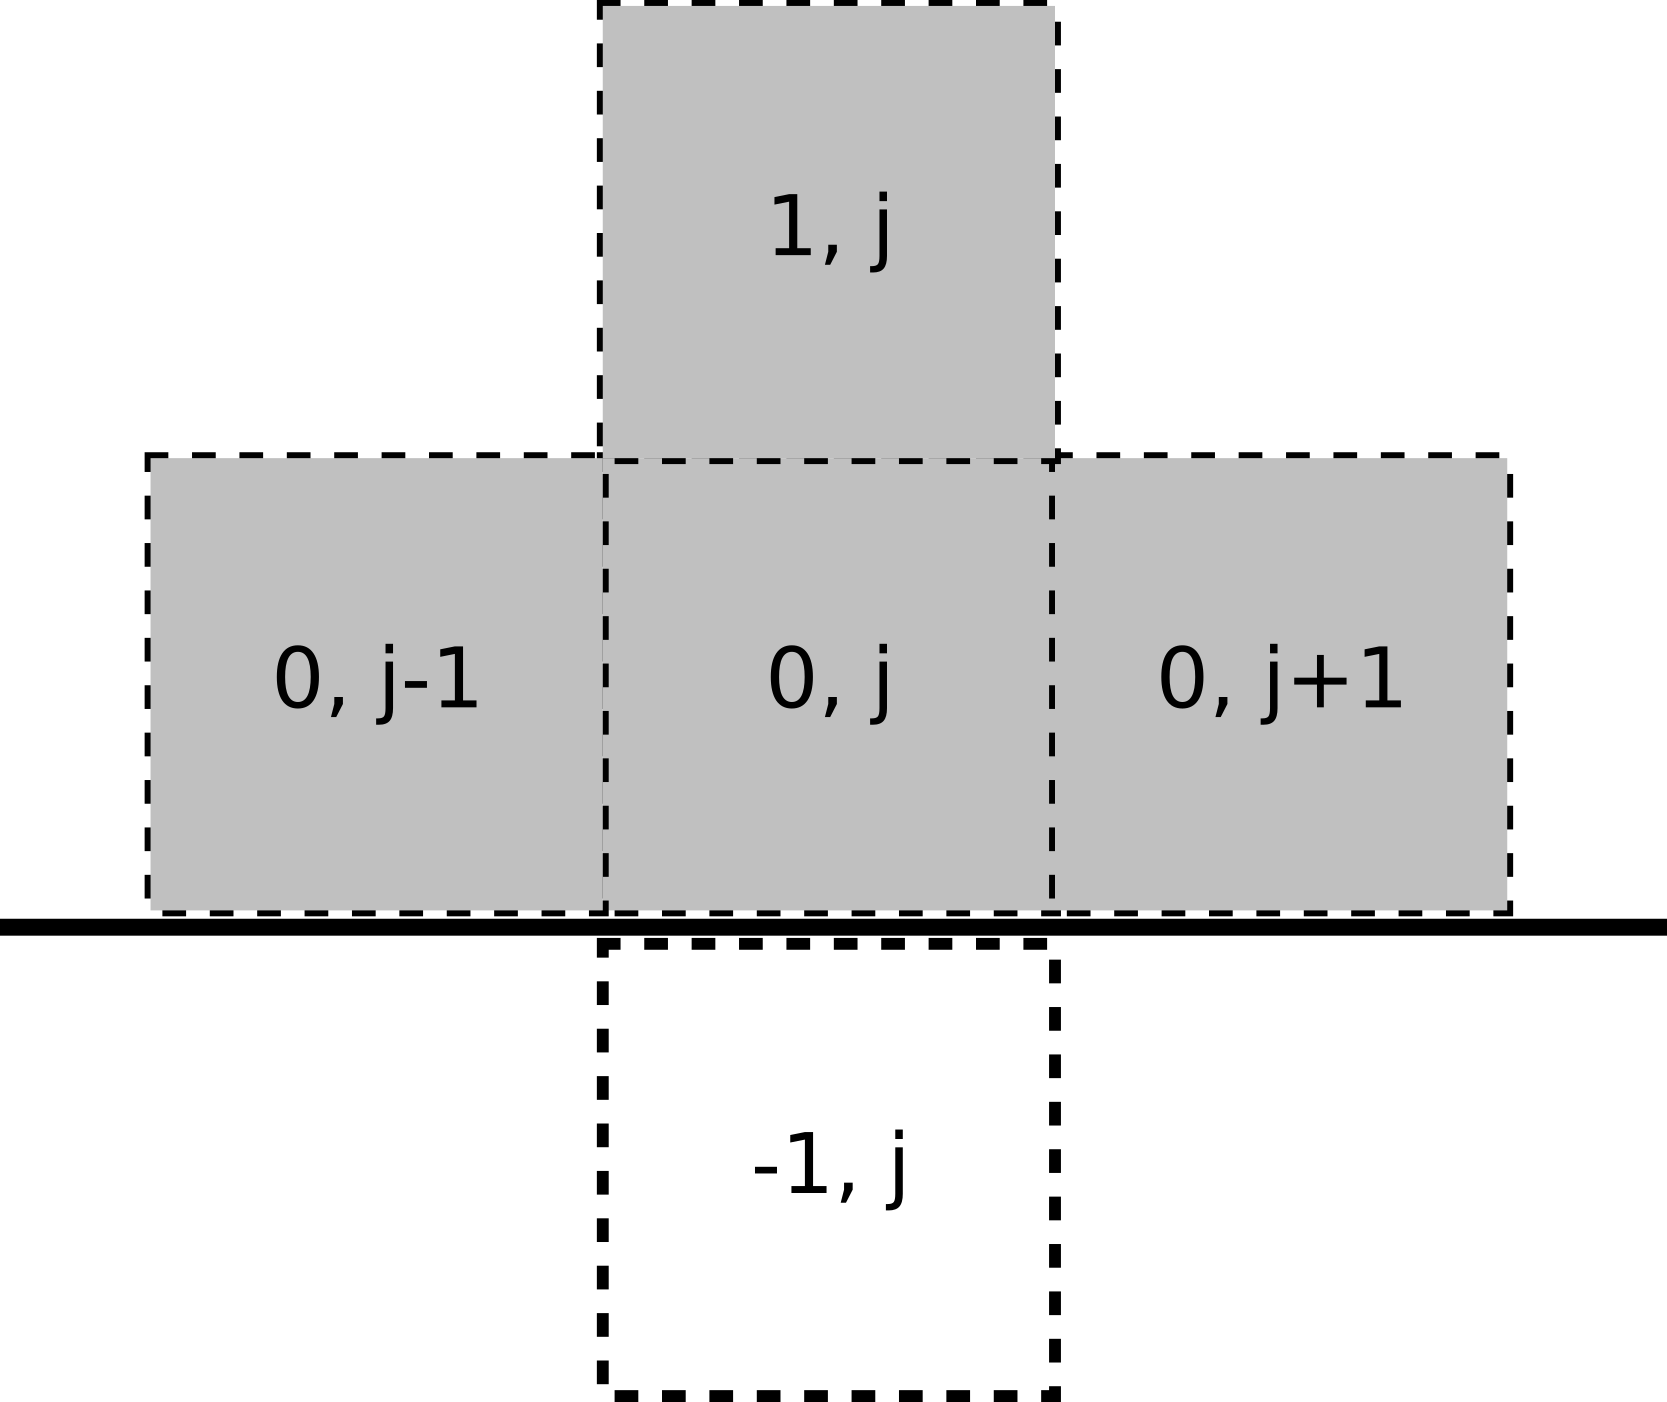
\includegraphics[width=3in]{Figures/imaginary-grid.png}
\caption[Imaginary-grid]
{
Use boundary condition to generate imaginary grid nodes.
}
\label{fig:im-grid}
\end{center}
\end{figure}
%
Formally, the boundary conditions at $y=0$ can be written as
$$
\frac{\psi_{0, j}-\psi_{-1, j}}{h} = 0, \ \frac{\psi_{0, j+1}-\psi_{0, j}}{h} = 0
$$
Similarly, at $y=1$
$$
\frac{\psi_{N, j}-\psi_{N-1, j}}{h} = 0, \ \frac{\psi_{N-1, j+1}-\psi_{N-1, j}}{h} = 0
$$
%
Apply the conditions above to the 5-point discretization scheme in Eq.~\ref{eq:discrete-laplacian-approx}, we have
%
\begin{equation}\label{eq:discrete-bc-y0} % discrete BC at y=0
\begin{split}
(\nabla^2\psi)_{0, j} & = \frac{\psi_{1, j} + \psi_{0, j+1} - 4\psi_{0, j} + \psi_{-1, j} + \psi_{0, j-1}}{h^2} \\
  & = \frac{\psi_{1, j} - \psi_{0, j}}{h^2}
\end{split}
\end{equation}
%
\begin{equation}\label{eq:discrete-bc-y1} % discrete BC at y=1
\begin{split}
(\nabla^2\psi)_{N-1, j} & = \frac{\psi_{N, j} + \psi_{N-1, j+1} - 4\psi_{N-1, j} + \psi_{N-2, j} + \psi_{N-1, j-1}}{h^2} \\
  & = \frac{\psi_{N-1, j} - \psi_{N-2, j}}{h^2}
\end{split}
\end{equation}

%
Eqs.~\ref{eq:discrete-bc-y0} and \ref{eq:discrete-bc-y1} holds for $j = 0, 1, \dots, N-1$ since the evaluation of the Laplacian does not require a derivative in $x$ direction.

To impose the periodic boundary conditions at $x=0$ and $x=1$ (i.e. $j=0$ and $j=N-1$), we start by noticing that
%
\begin{equation}\label{eq:e-periodic-bc}
\psi_{i, -1} = \psi_{i, N-1}, \ \psi_{i, N} = \psi_{i, 0}
\end{equation}
%
Eq.~\ref{eq:e-periodic-bc} only considers the very edge of the boundary, but is already sufficient for performing the 5-point discretization:
\begin{equation}\label{eq:discretized-periodic-bc}
\begin{split}
(\nabla^2\psi)_{i, 0} & = \frac{\psi_{i+1, 0} + \psi_{i, 1} - 4\psi_{i, 0} + \psi_{i-1, 0} + \psi_{i, N-1}}{h^2} \\
(\nabla^2\psi)_{i, N-1} & = \frac{\psi_{i+1, N-1} + \psi_{i, 0} - 4\psi_{i, N-1} + \psi_{i-1, N-1} + \psi_{i, N-2}}{h^2}
\end{split}
\end{equation}
%
Eq.~\ref{eq:discretized-periodic-bc} hold for $i=1, 2, \dots, N-2$. Up to here, we have the discretized formulation for all the nodes in the field, and we are ready to go about solving the equation!

Using Eqs.~\ref{eq:discrete-bc-y0}, \ref{eq:discrete-bc-y1} and \ref{eq:e-periodic-bc}, we can construct the matrix $\bm{A}$ for the linear system. Usually, $\bm{A}$ is very large ($N^2\times N^2$) and sparse (with only a few diagnals with nonzero numbers). Therefore, we construct sparse matrix to save computational power.
Fig.~\ref{fig:A-matrix} shows an illustration of the matrix $\bm{A}$, where 7 nonzero diagnals need to be constructed. Table.~\ref{tab:diagnal-comp} shows the compositions of the 7 nonzero diagnals.
%
\begin{figure}[h]
\begin{center}
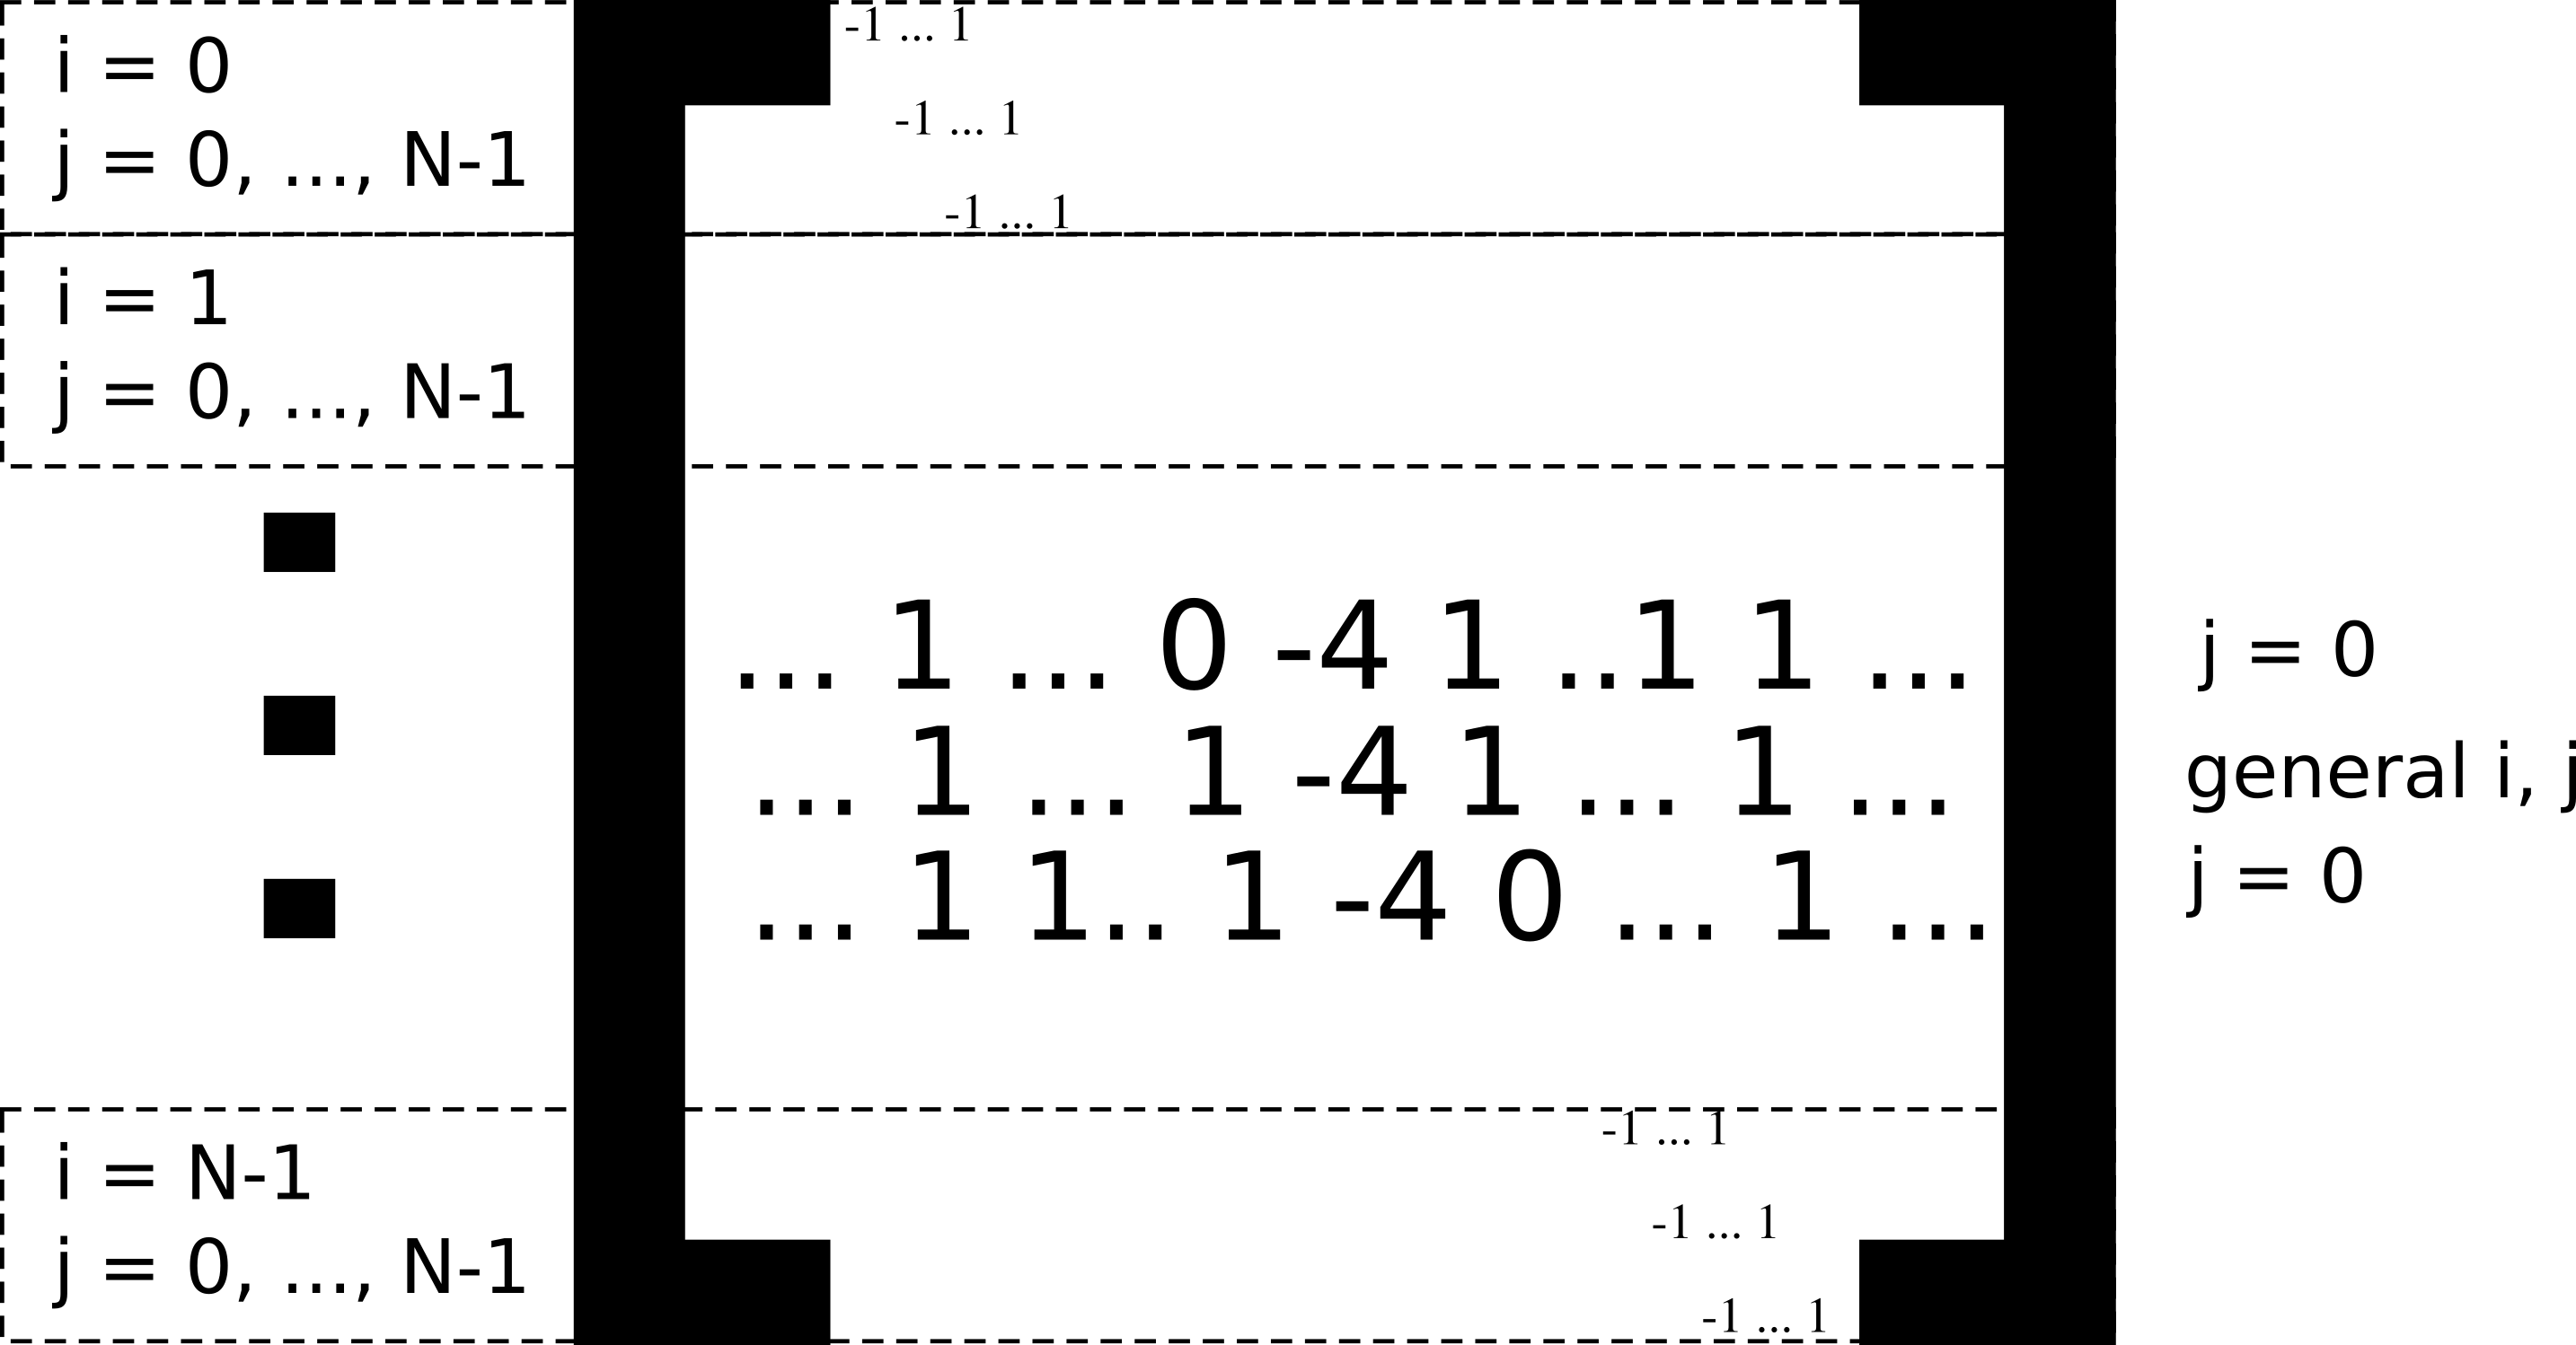
\includegraphics[width=3in]{Figures/A-matrix.png}
\caption[A-matrix]
{
An illustration of the linear system.
}
\label{fig:A-matrix}
\end{center}
\end{figure}

% construct a table listing the compositions of the 7 diagnals
\begin{table}
  \begin{center}
    \begin{tabular}{l|l|l}
\hline
Name & Position & Composition \\
\hline
\tt e\_3 & $-N$ & $[1]\times (N-1)N + [-1]\times N$ \\
\tt e\_2 & $-N+1$ & $[0]+([0]\times(N-1)+[1])\times (N-2)+[0]\times N$ \\
\tt e\_1 & $-1$ & $[0]\times (N-1)+([0]+[1]\times( N-1))\times(N-2)+[0]\times N$ \\
\tt e   & $0$ & $[-1]\times N + [-4]\times(N-2)N + [1]\times N$ \\
\tt e1  & $1$ & $[0]\times N + ([1]\times(N-1)+[0])\times(N-2) + [0]\times(N-1)$ \\
\tt e2  & $N-1$ & $[0]\times N + ([1]+[0]\times(N-1))\times(N-2)+[0]$ \\
\tt e3  & $N$ & $[1]\times(N-1)N$ \\
\hline
    \end{tabular}
    \caption{Nonzero diagnals in $\bm{A}$.}
    \label{tab:diagnal-comp}
  \end{center}
\end{table}

Now we have everything we need to solve for the function $\psi$ in Eq.~\ref{eq:poisson}, or for the $\bm{x}$ in the formulation in Eq.~\ref{eq:linear-system}. We test the method by constructing a vorticity field $\bm{\omega}$ and solve for $\psi$. Figure~\ref{fig:result} shows the flow fields corresponding to a random and a sinusoidal vorticity fields. \\[1em]
%
\begin{figure}[h]
\begin{center}
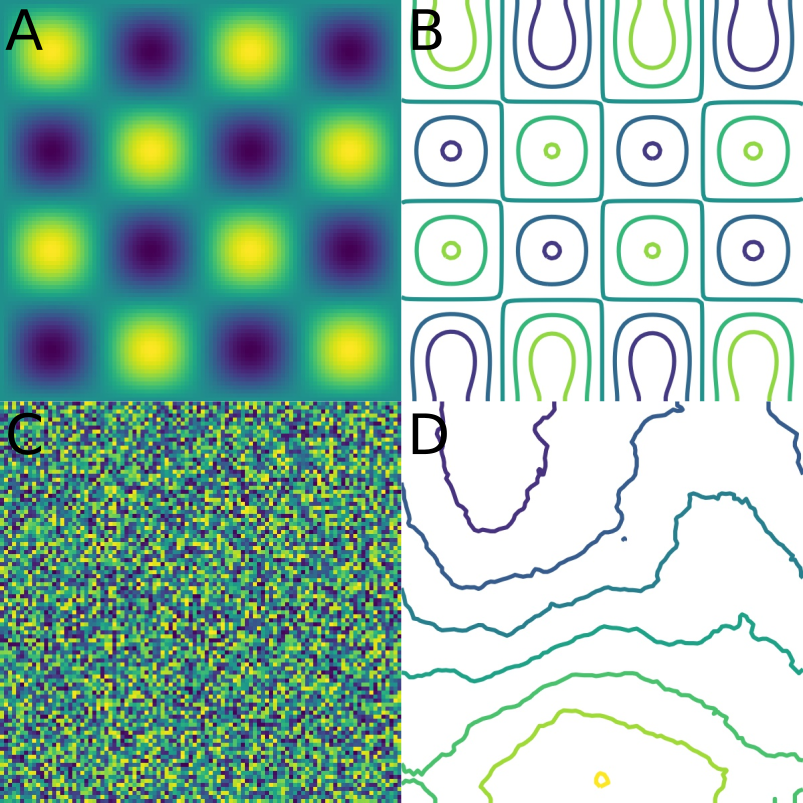
\includegraphics[width=3in]{Figures/result.png}
\caption[result]
{
Examle solutions of the Poisson equation.
}
\label{fig:result}
\end{center}
\end{figure}

\noindent\textbf{Supplemental Content} \\[0px]
[1] \href{https://github.com/ZLoverty/DD/blob/main/Simulation/Poisson%20equation.ipynb}{Implementation in Jupyter notebook}

\end{document}
